\begin{figure}[H]
    \centering
    \begin{tikzpicture}
        \scriptsize

        \node at (0,2) (A) {Discretization in different dimensions};
        \node at (-4,1.4) (B) {1D};
        \node at (0,1.4) (C) {2D};
        \node at (4,1.4) (D) {3D};

        \draw[->] (A) -- (C);
        \draw[->] (A) -- (-4,2) -- (B);
        \draw[->] (A) -- (4,2) -- (D);

        \node at (-4,0.7) (E) {
\includegraphics[width=0.218\textwidth]{Immagini/element-1D.png}};
        \node at (0,0.7) (F) {\includegraphics[width=0.2\textwidth]{Immagini/elements-2D.png}};
        \node at (4,0.68) (G) {\includegraphics[width=0.22\textwidth]{Immagini/elements-3D.png}};

        \visible<2->{\node at (-4,-1.8) (H) {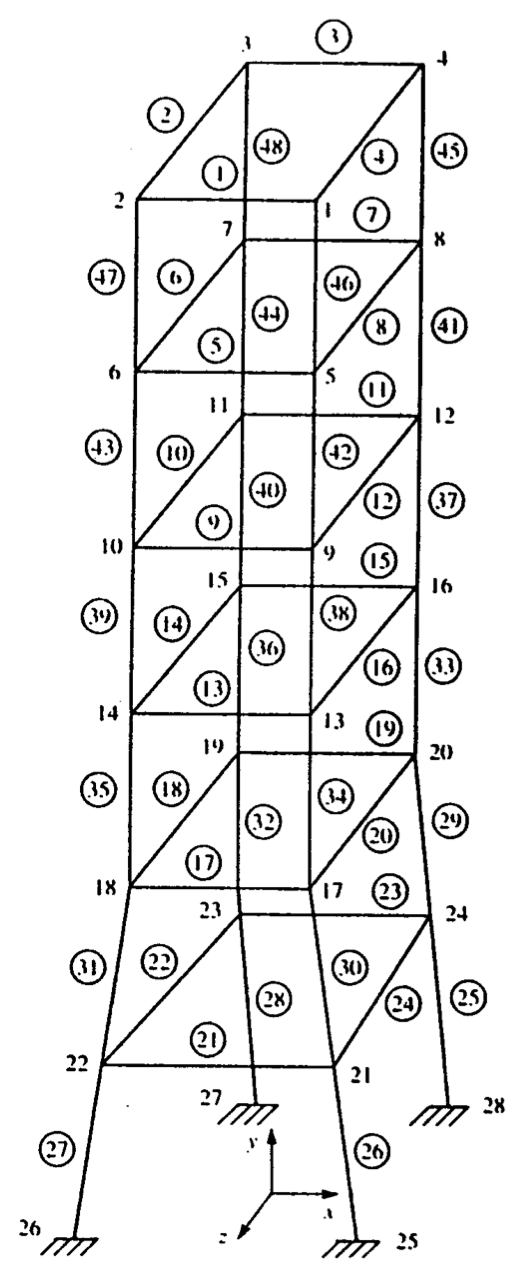
\includegraphics[width=0.14\textwidth]{Immagini/frame-elements.png}};
        \node at (-0.1,-1.9) (I) {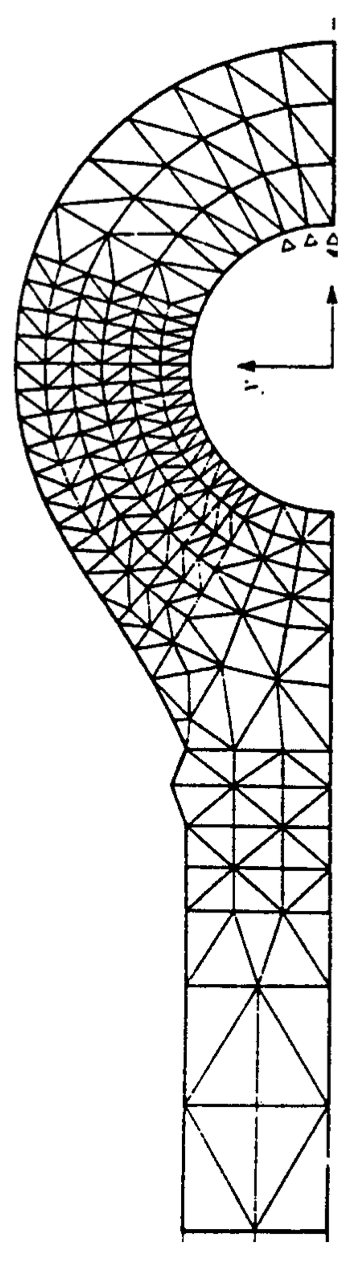
\includegraphics[width=0.1\textwidth]{Immagini/triangular elements.png}};
        \node at (3.78,-1.95) (J) {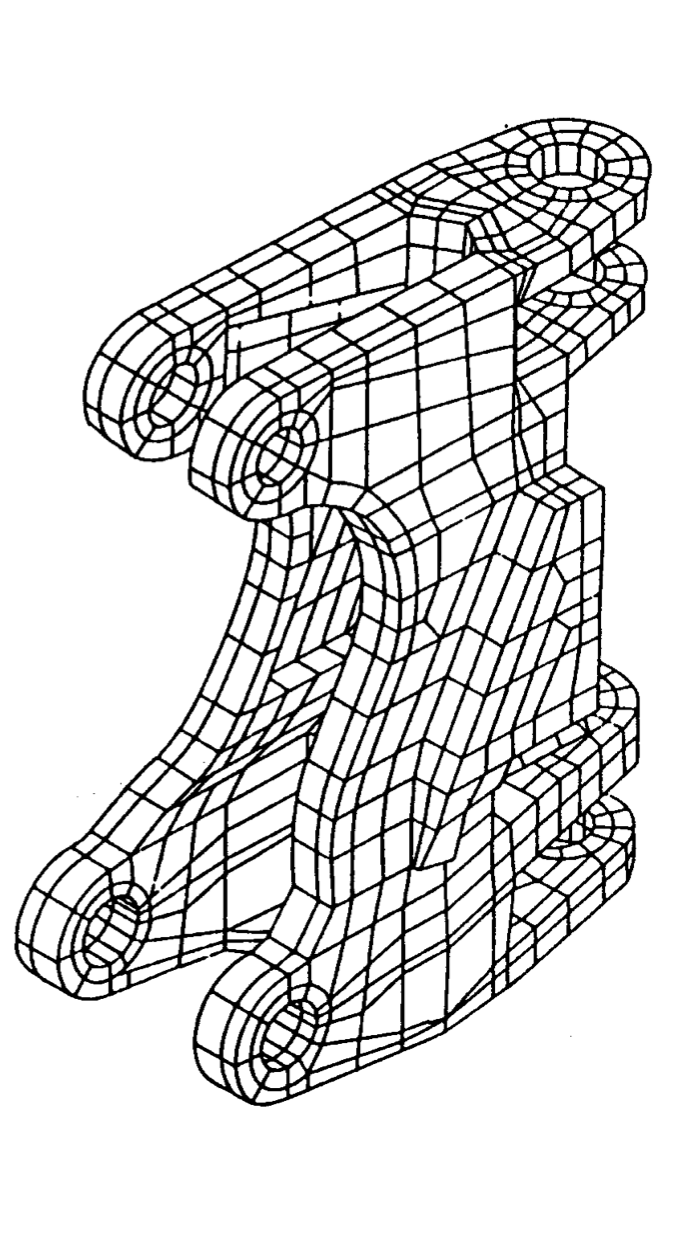
\includegraphics[width=0.21\textwidth]{Immagini/brick-elements.png}};

        \node at (-4,-4.1) (K) {\textbf{Frame \textcolor{BrickRed}{elements}}};
        \node at (0,-4.1) (L) {\textbf{Triangular \textcolor{BrickRed}{elements}}};
        \node at (4,-4.1) (M) {\textbf{Brick \textcolor{BrickRed}{elements}}};}

        \visible<3->{\draw[decorate, decoration={brace, amplitude=8pt, raise=2pt}] (5.25,-4.25) -- (-5.25,-4.25);

        \node at (0,-4.85) (N) {\textbf{Finite \textcolor{BrickRed}{Element} Method}};}

        \normalsize
    \end{tikzpicture}
\end{figure}